\documentclass[tikz, border=10pt]{standalone}
\usepackage{pgfplots}
\pgfplotsset{compat=1.18}

\begin{document}
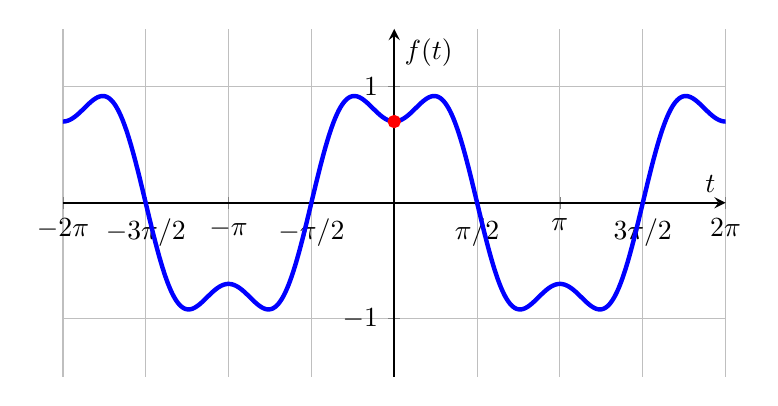
\begin{tikzpicture}
    \begin{axis}[
        width=10cm, height=6cm,
        axis lines=middle,
        xlabel={$t$}, ylabel={$f(t)$},
        ymin=-1.5, ymax=1.5,
        xmin=-2*pi, xmax=2*pi,
        xtick={-6.28, -4.71, -3.14, -1.57, 0, 1.57, 3.14, 4.71, 6.28},
        xticklabels={$-2\pi$, $-3\pi/2$, $-\pi$, $-\pi/2$, 0, $\pi/2$, $\pi$, $3\pi/2$, $2\pi$},
        grid=both,
        samples=400,
        domain=-2*pi:2*pi,
        thick
    ]
        % f(t) = cos(t) - 0.3*cos(3t)
        \addplot[blue, ultra thick] {cos(deg(x)) - 0.3*cos(deg(3*x))};
        
        \addplot[only marks, mark=*, red] coordinates {(0, 0.7)};
    \end{axis}
\end{tikzpicture}
\end{document}
